\documentclass[a4paper,twocolumn]{article} % Document type

\ifx\pdfoutput\undefined
    %Use old Latex if PDFLatex does not work
   \usepackage[dvips]{graphicx}% To get graphics working
   \DeclareGraphicsExtensions{.eps} % Encapsulated PostScript
 \else
    %Use PDFLatex
   \usepackage[pdftex]{graphicx}% To get graphics working
   \DeclareGraphicsExtensions{.pdf,.jpg,.png,.mps} % Portable Document Format, Joint Photographic Experts Group, Portable Network Graphics, MetaPost
   \pdfcompresslevel=9
\fi
\usepackage{multirow}
\usepackage{subcaption}
\usepackage{amsmath,amssymb}   % Contains mathematical symbols
\usepackage[ansinew]{inputenc} % Input encoding, identical to Windows 1252
\usepackage[english]{babel}    % Language
%\usepackage[round,authoryear]{natbib}  %Nice author (year) citations
\usepackage[square,numbers]{natbib}     %Nice numbered citations
%\bibliographystyle{unsrtnat}           %Unsorted bibliography
\bibliographystyle{plainnat}            %Sorted bibliography

\addtolength{\topmargin}{-30mm}% Removes 30mm from the top margin
\addtolength{\textheight}{30mm}% Adds it to the text height


\begin{document}               % Begins the document

\title{Reproducing Sequential Attention for Feature Selection}
\author{Gary Wang, Hank Lai \\ N16132087, N16132079 \\ n16132087@gs.ncku.edu.tw, n16132079@gs.ncku.edu.tw} 
%\date{2010-10-10}             % If you want to set the date yourself.

\maketitle                     % Generates the title




%%%%%%%%%%%%%%%%%%%%%%%%%%%%%%%%%%%%%%%%%%%%%%%%%%%%%%%%%%%%%%%%%%%%%%%%%%%%%%%%%%%
% Instructions regarding the report
%%%%%%%%%%%%%%%%%%%%%%%%%%%%%%%%%%%%%%%%%%%%%%%%%%%%%%%%%%%%%%%%%%%%%%%%%%%%%%%%%%%

\section{Introduction}

Feature selection is essential for improving interpretability, generalization, and efficiency in high-dimensional learning tasks.
 However, As noted in a review by Nordling (2013, Chapter 5.2) have noted, it remains a challenging problem due to 
computational limits and sensitivity to noise. Classical methods such as LASSO and greedy search either fail to capture feature interactions or lack robustness.

Sequential Attention (SA)~\cite{yasuda2023} proposes a novel attention-based relaxation of greedy selection that models conditional importance adaptively. 
In this study, we aim to reproduce SA and evaluate whether it consistently outperforms classical methods 
like Sequential LASSO and Group LASSO.


\section{Methods}
%\subsection{Sequential Attention Algorithm}
% Description of algorithm, possibly Algorithm 1 from paper
\subsection{Dice Coefficient}
The Dice coefficient measures the similarity between two binary masks. It is defined as:
\begin{equation}
    \mathrm{Dice}(A, B) = \frac{2|A \cap B|}{|A| + |B|},
\end{equation}
where $A$ and $B$ are the sets of selected and reference features, respectively. A Dice score closer to 1 indicates higher overlap. In our study, we use it to select the best-performing seed for each method.
\subsection{Statistical Testing (p-value).}
To assess the statistical significance of performance differences, we conduct $t$-tests. For the model using all features , we apply a one-sample $t$-test to compare the accuracy against the reference value reported in the original paper. For the case with feature selection ($k=50$), we use a two-sample $t$-test to compare the accuracies of the selected and unselected feature models.
\begin{equation}
    H_0: \mu = \mu_0,
\end{equation}
where $\mu$ is the sample mean from repeated trials, and $\mu_0$ is the reference mean.

For comparing two methods directly, we use a two-sample $t$-test assuming equal variances:
\begin{equation}
    H_0: \mu_1 = \mu_2,
\end{equation}
to test whether the difference in means is statistically significant. In both tests, a low p-value (e.g., $< 0.05$) indicates that the observed difference is unlikely due to random chance.

\section{Results}
Small-scale experiments evaluate feature selection methods on benchmark datasets using a simple neural network with 50 selected features.
\subsection{Visuallization Of Selected MNIST Features}

As shown in Table~\ref{tab:dice_results}, we used the Dice coefficient to identify the most similar image. As illustrated in Figure~\ref{fig:feature_masks}, our results appear visually comparable to those of Yasuda (2023).; however, the Dice scores remain suboptimal (where values closer to 1 indicate higher similarity). Nevertheless, we consider the quantitative evaluation to be complete.
\begin{table}[ht]
    \centering
    \begin{tabular}{lcc}
        \hline
        \textbf{Method} & \textbf{Seed} & \textbf{Dice} \\
        \hline
        SA    & 3 & 0.1800 \\
        LLY   & 3 & 0.1600 \\
        GL    & 1 & 0.4200 \\
        SEQL  & 2 & 0.1600 \\
        OMP   & 1 & 0.2600 \\
        \hline
    \end{tabular}
    \caption{Dice coefficients for the best seed selected by each method.}
    \label{tab:dice_results}
\end{table}
\begin{figure*}[h!]
    \centering
    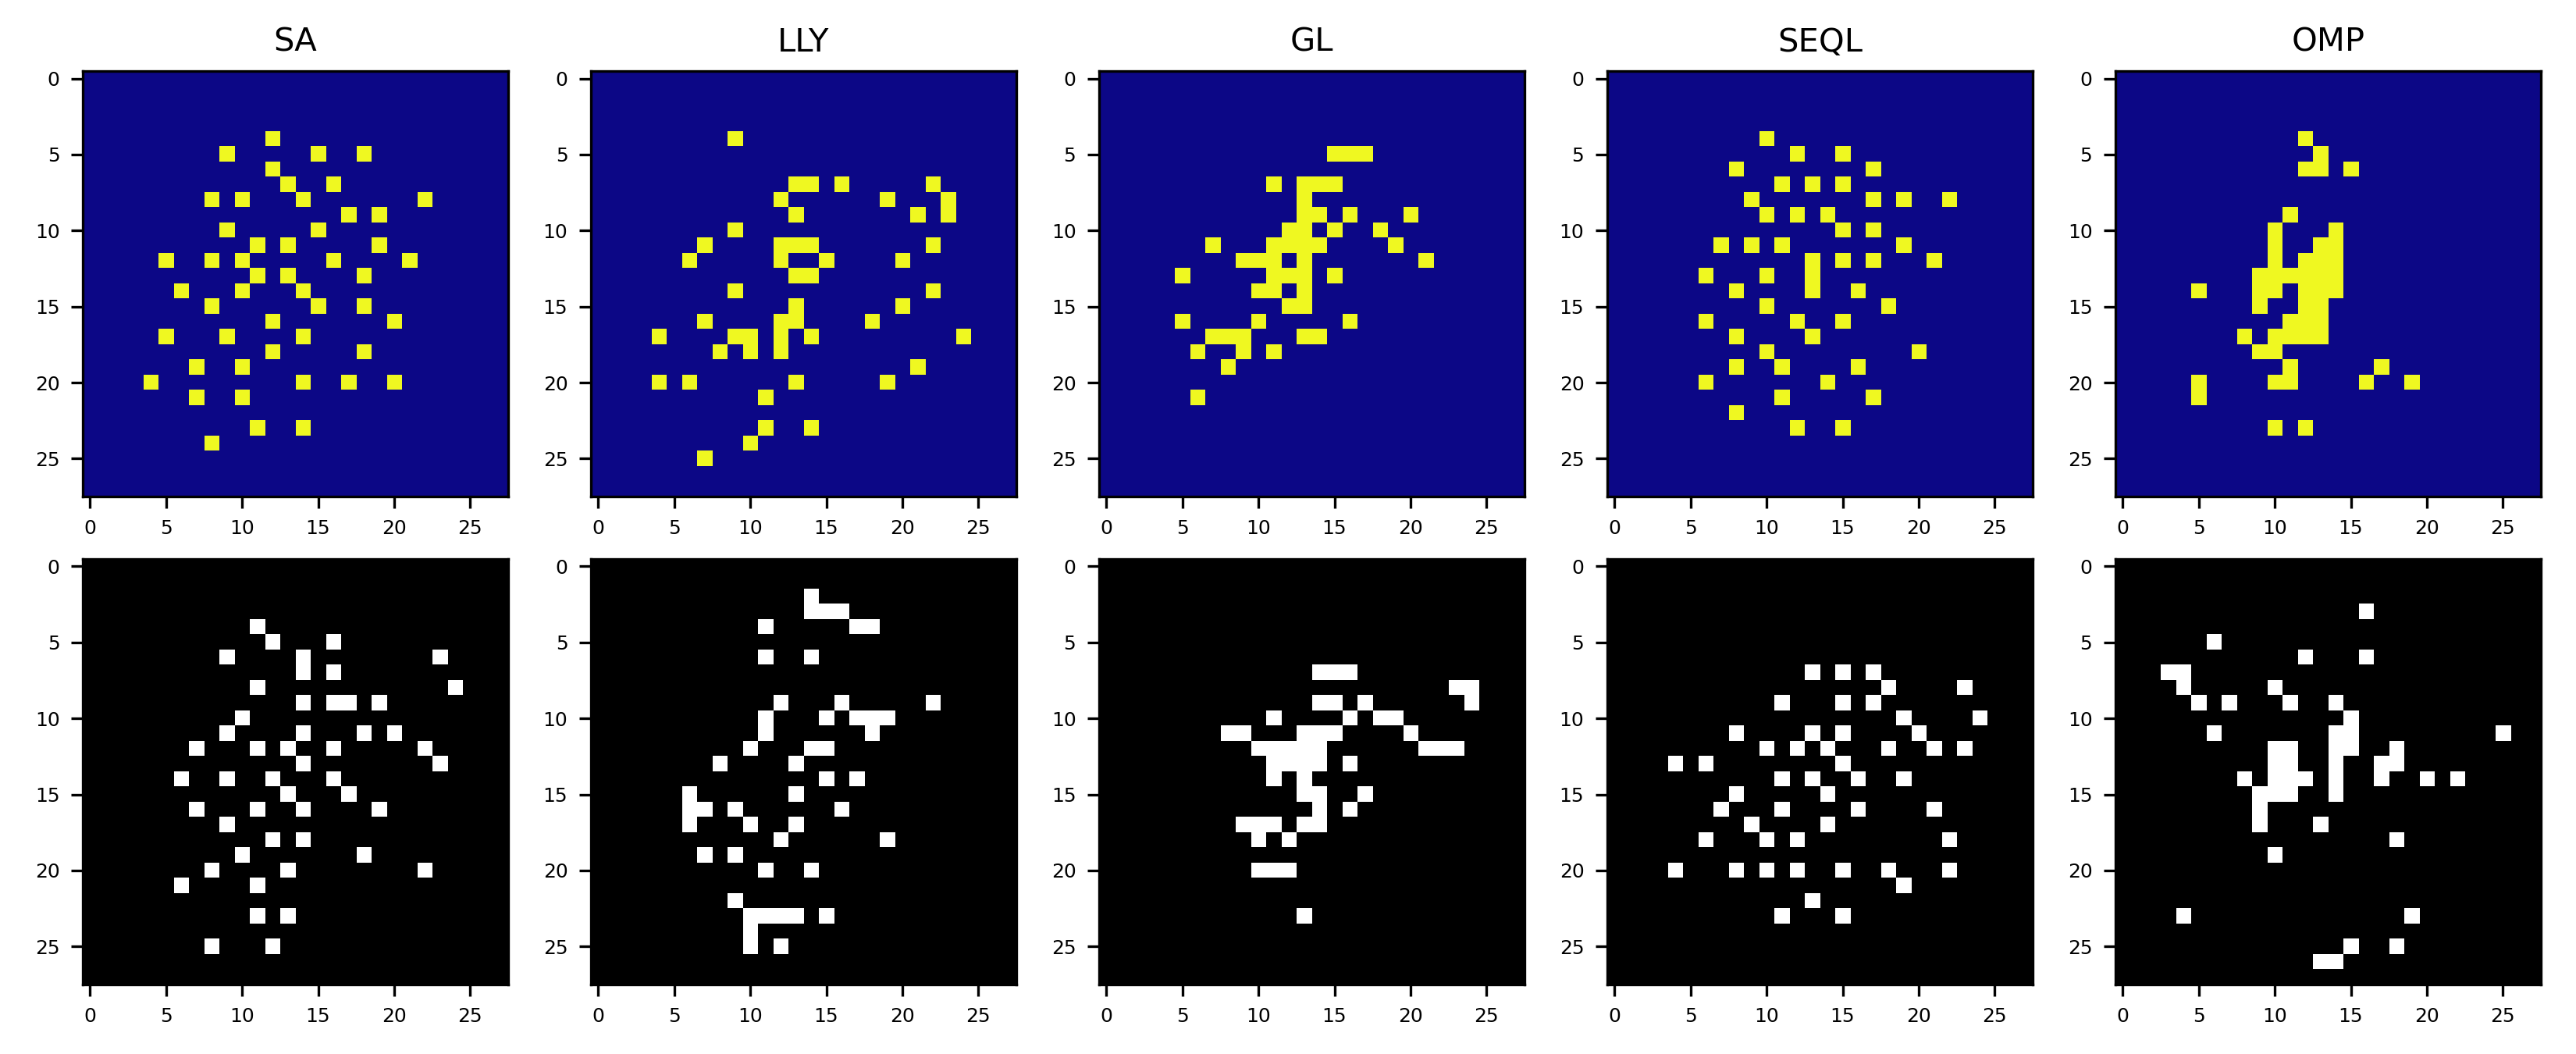
\includegraphics[width=\textwidth]{figures/all_methods_with_axis.png}
    \caption{Top row: feature masks from Yasuda et al. (2023); bottom row: our reproduced result for each method. Axes denote feature indices.}
    \label{fig:feature_masks}
\end{figure*}
%\subsection{Dataset Overview}

\subsection{Statistical Validation}
% t-test or p-value results table if needed
\subsubsection*{With Feature Selection (Top 50 Features)}
In Table~\ref{tab:methodwise-pval}, we observe that for certain method-dataset combinations, the $p$-value exceeds 0.5, suggesting no statistically significant difference—this supports the quantitative reproducibility of the results. On the other hand, even in cases where the $p$-value is below 0.5, the corresponding accuracies in Table~\ref{tab:accuracy-ours-vs-paper} remain very close to the original results. Therefore, we argue that our reproduction successfully achieves qualitative agreement with the original findings.
\begin{table}[ht]
\centering
\scriptsize
\begin{tabular}{lccccc}
\hline
\textbf{Dataset} & \textbf{SA} & \textbf{LLY} & \textbf{GL} & \textbf{SL} & \textbf{OMP} \\
\hline
Mice     & \textbf{0.9276} & 0.0220 & 0.0227 & 0.0673 & \textbf{0.5906} \\
MNIST    & 0.0961 & 0.0013 & 0.0002 & 0.0000 & 0.0607 \\
Fashion  & 0.0105 & \textbf{0.8313} & 0.0031 & 0.0007 & 0.0000 \\
ISOLET   & 0.0551 & \textbf{0.6804} & 0.0003 & 0.3600 & 0.0037 \\
COIL-20  & 0.3895 & \textbf{0.5901} & 0.0093 & 0.1437 & 0.3519 \\
Activity & \textbf{0.7448} & 0.3194 & \textbf{0.7802} & 0.0034 & 0.2388 \\
\hline
\end{tabular}
\caption{p-values comparing reproduced results with Yasuda (2023) for each method .}
\label{tab:methodwise-pval}
\end{table}

\begin{table*}[ht]
\centering
\resizebox{\textwidth}{!}{%
\begin{tabular}{llcccccc}
\hline
\textbf{Dataset} &  & \textbf{SA} & \textbf{LLY} & \textbf{GL} & \textbf{SL} & \textbf{OMP} & \textbf{CAE} \\
\hline
\multirow{2}{*}{Mice Protein} &
\textit{Yasuda (2023)} & 
0.993 $\pm$ 0.008 & 0.981 $\pm$ 0.005 & 0.985 $\pm$ 0.005 & 0.984 $\pm$ 0.008 & 0.994 $\pm$ 0.008 & 0.956 $\pm$ 0.012 \\
& \textit{Reproduced} & 
\textbf{0.993 $\pm$ 0.008} & 0.992 $\pm$ 0.007 & 0.994 $\pm$ 0.006 & 0.994 $\pm$ 0.008 & \textbf{0.992 $\pm$ 0.007} & -- \\
\hline
\multirow{2}{*}{MNIST} &
\textit{Yasuda (2023)} & 
0.956 $\pm$ 0.002 & 0.944 $\pm$ 0.001 & 0.937 $\pm$ 0.003 & 0.959 $\pm$ 0.001 & 0.912 $\pm$ 0.004 & 0.909 $\pm$ 0.007 \\
& \textit{Reproduced} & 
0.954 $\pm$ 0.001 & 0.938 $\pm$ 0.002 & 0.926 $\pm$ 0.003 & 0.952 $\pm$ 0.001 & 0.892 $\pm$ 0.018 & -- \\
\hline
\multirow{2}{*}{MNIST-Fashion} &
\textit{Yasuda (2023)} & 
0.854 $\pm$ 0.003 & 0.843 $\pm$ 0.005 & 0.834 $\pm$ 0.004 & 0.854 $\pm$ 0.003 & 0.829 $\pm$ 0.008 & 0.839 $\pm$ 0.003 \\
& \textit{Reproduced} & 
0.846 $\pm$ 0.004 & \textbf{0.844 $\pm$ 0.004} & 0.842 $\pm$ 0.003 & 0.845 $\pm$ 0.003 & 0.768 $\pm$ 0.012 & -- \\
\hline
\multirow{2}{*}{ISOLET} &
\textit{Yasuda (2023)} & 
0.920 $\pm$ 0.006 & 0.866 $\pm$ 0.012 & 0.906 $\pm$ 0.006 & 0.920 $\pm$ 0.003 & 0.727 $\pm$ 0.026 & 0.893 $\pm$ 0.011 \\
& \textit{Reproduced} & 
0.927 $\pm$ 0.005 & \textbf{0.869 $\pm$ 0.010} & \textbf{0.887 $\pm$ 0.005} & 0.923 $\pm$ 0.007 & 0.808 $\pm$ 0.035 & -- \\
\hline
\multirow{2}{*}{COIL-20} &
\textit{Yasuda (2023)} & 
0.997 $\pm$ 0.001 & 0.994 $\pm$ 0.002 & 0.997 $\pm$ 0.004 & 0.988 $\pm$ 0.005 & 0.967 $\pm$ 0.014 & 0.972 $\pm$ 0.007 \\
& \textit{Reproduced} & 
\textbf{0.994 $\pm$ 0.008} & \textbf{0.992 $\pm$ 0.006} & \textbf{0.991 $\pm$ 0.002} & \textbf{0.992 $\pm$ 0.005} & \textbf{0.976 $\pm$ 0.016} & -- \\
\hline
\multirow{2}{*}{Activity} &
\textit{Yasuda (2023)} & 
0.931 $\pm$ 0.004 & 0.897 $\pm$ 0.025 & 0.933 $\pm$ 0.002 & 0.931 $\pm$ 0.003 & 0.905 $\pm$ 0.013 & 0.921 $\pm$ 0.001 \\
& \textit{Reproduced} & 
\textbf{0.930 $\pm$ 0.003} & \textbf{0.908 $\pm$ 0.010} & \textbf{0.934 $\pm$ 0.008} & 0.917 $\pm$ 0.006 & \textbf{0.887 $\pm$ 0.029} & -- \\
\hline
\end{tabular}
}
\caption{Accuracy comparison: Yasuda (2023) vs. reproduced results across all datasets.}
\label{tab:accuracy-ours-vs-paper}
\end{table*}

\begin{table}[ht]
\centering
\resizebox{\linewidth}{!}{%
\begin{tabular}{lccccc}
\hline
\textbf{Dataset} & \textbf{Our results} & \textbf{Lemhadri} & \textbf{p-value} & \textbf{Yasuda} & \textbf{p-value} \\
\hline
Mice Protein     & \textbf{0.989 $ \pm $ 0.008} & 0.990 & \textbf{0.7623} & 0.963 & 0.0017 \\
MNIST            & 0.973 $ \pm $ 0.001 & 0.928 & 0.0000 & 0.953 & 0.0000 \\
MNIST-Fashion    & 0.874 $ \pm $ 0.003 & 0.833 & 0.0000 & 0.869 & 0.0297 \\
ISOLET           & 0.950 $ \pm $ 0.003 & 0.953 & 0.1269 & 0.961 & 0.0015 \\
COIL-20          & 0.994 $ \pm $ 0.002 & 0.996 & 0.1381 & 0.986 & 0.0005 \\
Activity         & 0.942 $ \pm $ 0.002 & 0.853 & 0.0000 & 0.954 & 0.0002 \\
\hline
\end{tabular}
}
\caption{Comparison of accuracy using all features. p-values are from one-sample t-tests against Lemhadri (2021)~\cite{lemhadri2021lassonet} and Yasuda (2023)'s reported means.}
\label{tab:all-feature-pval}
\end{table}
\section{Discussion}
% Analysis of differences, strengths, weaknesses, generalization, possible error sources


\subsection{ Large-scale experiments}
We encountered difficulties reproducing the large-scale experiment presented in Figure 4 of the original paper. Specifically, the Criteo Click dataset used in that experiment requires approximately 1TB of disk space. 
Due to hardware limitations on both our local machines and available servers, we were unable to process and store the full dataset. 
As a result, we were not able to reproduce the large-scale results associated with this figure.

\section{Conclusion}
% Summary of what was reproduced and whether claims hold

\bibliographystyle{ieeetr}
\bibliography{references}


% Optionally include appendix
\clearpage
\appendix
\section*{Appendix}
\section{Hyperparameters}
% Learning rate, batch size, etc.

\section{Additional Figures}
% Supplementary plots

\end{document}      % End of the document
